%
% File XCS224U_final_paper.tex
%

\documentclass[11pt,a4paper]{article}
\usepackage[hyperref]{acl2020}
\usepackage{times}
\usepackage{latexsym}
\usepackage{graphicx}
\renewcommand{\UrlFont}{\ttfamily\small}

% This is not strictly necessary, and may be commented out,
% but it will improve the layout of the manuscript,
% and will typically save some space.
\usepackage{microtype}

\aclfinalcopy % Uncomment this line for the final submission
%\def\aclpaperid{***} %  Enter the acl Paper ID here

%\setlength\titlebox{5cm}
% You can expand the titlebox if you need extra space
% to show all the authors. Please do not make the titlebox
% smaller than 5cm (the original size); we will check this
% in the camera-ready version and ask you to change it back.

\newcommand\BibTeX{B\textsc{ib}\TeX}

\title{Colors in Context: Grounded Language Understanding using Vision and Transformer Embeddings}

\author{
  Anton Gochev \\
  \texttt{gochev.anton@gmail.com} \\
  \And
  Jaro Habr \\
  \texttt{jaro.habr@gmail.com} \\
  \AND
  Yan Jiang \\
  \texttt{enaj1125@gmail.com} \\
  \And
  Samuel Kahn \\
  \texttt{samuelkahn@berkeley.edu} \\
}

\date{}

\begin{document}
\maketitle

\begin{abstract}

\begin{itemize}
  In this work we present a new model for a grounded communication task; identifying colors  generated from descriptions. This task uses two recurrent neural network cells which act as the speaker generating utterances. We build on previous work and introduce two novel methods for embedding our recurrent neural network inputs; a convolutional encoder for colors and a transformer network for encoding utterances. We show that coupling these two encoders with a recurrent sequence-to-sequence architectures can sometimes achieve state-of-the-art results in both listener accuracy and BLEU score, but the gains are often minimal with a much greater computational profile. In addition, our paper demonstrates that using complex encoders such as transformers or convolutional neural networks on small high dimensional datasets don't clearly outperform simpler models such as a Fourier Transform or GLoVe.


% \begin{itemize}
%   \item define current proposal, situate in context
%   \item summarize core findings
%   \item identify significance of work
% \end{itemize}

\end{abstract}
\section{Introduction}

Human language is highly contextual and often presumes prior knowledge of a given topic. Meaning of words is mostly implicit and is inferred from context. Such interpretations are difficult for machine learning models as context is not only represented by words but it also assumes as a common world understanding \citep{monroe-2017-colors}. In reality, words can have different meanings in different contexts and hence cannot be represented with a single vector. This obvervation let to the introduction of contextual word representations based on word tokens and has been widely adopted by attention-based models and especially transformers like e.g. BERT, ELECTRA or XLNet \citep{smith-2019-contextual,vaswani-2017-attention}.

\par
Visual referring tasks like color or image descriptions are very suitable for language understanding tasks as they exercise this complex process of grounding in the environment and in our mental models of each other \citep{monroe-2017-colors, karpathy-2014-image_descriptions}.

\par
The central hypothesis of this paper is that rich color encondings as represented in convolutional neural networks (CNN) as well pre-trained and contextual word embeddings as used by attention based architectures such as transformers will help improve the performance on the color description task presented in \citep{monroe-2017-colors}. We hypothesize that those higher dimensional and more complex representations encode some useful information about the world and the given context from which a grounded communication task will be able to benefit.

\par
To address our hypothesis we build upon the sequence-to-sequence model presented by \citep{monroe-2017-colors}. As a first step we add a transfomer-based color descriptions encoder. Inspired by feature representations in computer vision, we then complement the model architecture with a ResNet color encoder pre-trained on ImageNet. This helps us to embed additional grounding information. To find the best performing setup, we finally perform a number of different operations on the transfomer encoder's hidden states, accompanied by a final fine-tuning along a defined hyperparameter space. The code of our work can be viewed on GitHub\footnote{\url{https://github.com/jhabr/xcs224u_final_paper}}.

\section{Related Work}

\begin{itemize}
  \item based on lit review
  \item organize paper into groups I want to cover =$>$ relation to my work
  \item for each group, articulate thematic unity, paper achievements =$>$ relation to my work =$>$ gives context, differentiation from prior work
\end{itemize}

As examples, we cite \citep{vaswani-2017-attention} to show you how papers with a DOI will appear in the bibliography.
We cite \citep{monroe-2017-colors} to show how papers without a DOI but with an ACL Anthology Identifier will appear in the bibliography.

\begin{itemize}
  \item Attention is all you need: \citep{vaswani-2017-attention}.
  \item Colors in Context: \citep{monroe-2017-colors}.
  \item Compositional Color Descriptions: \citep{monroe-2016-compositional}.
  \item GPT-3: \citep{brown-2020-gpt3}.
  \item Generating Image Descriptions: \citep{karpathy-2014-image_descriptions}.
  \item OpenAI Dall-E: \citep{openai-2020-dalle}.
  \item Huggingface: \citep{wolf-2019-huggingface}.
  \item Electra: \citep{clark-2020-electra}.
  \item XLNet: \citep{yang-2019-xlnet}.
  \item RoBERTa: \citep{liu-2019-roberta}.
  \item Contextual Word Representation: \citep{smith-2019-contextual}.
\end{itemize}

\section{Data}

We evaluate our models on the color dataset used in \citep{monroe-2017-colors}. This dataset was generated by playing reference games where the color descriptions were produced by human participants in the speaker role. On each round of the game, the speakers were presented with three color patches, one of which was selected to be the target color. The speakers were instructed to communicate this information to the listeners who were asked to click on one of the colors to complete the task \citep{monroe-2017-colors}.

\par
The dataset contains 49,025 examples in total and was split to train and test set with 46,994 and 2,031 examples respectively. Every dataset comprises examples containing three colors, one of them being the target color to be described and the other two being distractor colors. Every example belongs to one of three conditions: 1) \emph{close}, where all three colors are similar, 2) \emph{split}, where one of the colors is close to the target colors and 3) \emph{far}, where all three colors are far apart in the color space \citep{monroe-2017-colors}. Table \ref{table:colors} shows one example of each condition.

\begin{table}[ht]
\centering
\renewcommand{\arraystretch}{1}
\begin{tabular}{|l|l|l|}

  \hline
  Colors & Condition & Utterance \\
  \hline

\end{tabular}
\caption[Colors]{Colors...}
\label{table:colors}
\end{table}

\par
40.8\% of \emph{train} dataset color descriptions use one word, 59.2\% two or more with the majority being shorter than 14 words. All conditions are represented equally with 15,519 examples for the close condition, 15,693 examples for the split and 15,782 examples for the far condition. The train dataset is further divided using 90/10 split while training.

\par
The \emph{test} dataset has a slightly different composition. 40.2\% of the color descriptions use one word, 54.6\% use two words and only 5.2\% use three or more words. The conditions are represented with 633 examples for the close condition, 652 for the split condition and 746 for the far condition.
\section{Models}

This section describes the models in more detail.

\subsection{Target Architecture}
The following image depicts our target architecture developed for our experiments.

\begin{figure}[ht]
\centering
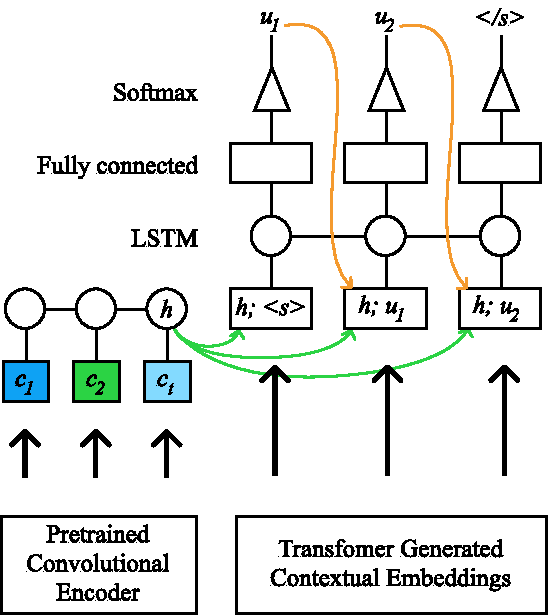
\includegraphics[width=\columnwidth]{assets/target_architecture.pdf}
\caption[Target Architecture]
{Target architecture with pretrained convolutional encoder and transformer generated contextual word embeddings.}
\label{overview}
\end{figure}

\par
The above architecture consists of three core components. The pretrained convolutional encoder is our method for extracting rich color embeddings. This could be any pretrained convolutional model such as \texttt{VGG19} or \texttt{Resnet152}, it just requires that we use one of the last hidden layers before the softmax projection as our encode color embeddings. We use the last layer of \texttt{ResNet18} in our experiments.

\par
The transformer generated contextual embeddings are any word embeddings generated by a transformer. This could be embeddings generated by \texttt{ELECTRA}, \texttt{XLNet}, \texttt{BERT} or any other transformer variants. These are used to encode the words into a semantic vector space where their project will be dependent on their context. Some descriptions are single words, thus contextual information will not be encoded.

\par
The generated color and contextual word embeddings are then brought together using a standard sequence-to-sequence architecture. The color embeddings are sent through an RNN unit such as a Gated Recurrent Unit or Long Short Term Memory Unit. The target color is sent through the RNN layer last so that it’s information encoded in the hidden state is \emph{closest} to the decoder. The decoder, another RNN unit,  then takes the hidden encoder's last hidden layer input and starts to decode the input utterance. For each timestep of the decoder we concatenate the target colors embedding, generated by the \texttt{ResNet18}, with the input word. Once the output RNN reaches its specified stop token we stop generating text.

\subsection{Experiment Setup}
To address our hypotheses we use different model compositions which are based on our target architecture.

\textbf{Baseline}:
As a baseline model, we use our implementation of the encoder-decoder architecture model based on a single layer of GRU for both the encoder and decoder. The colors are encoded using Fourier transformation.

\textbf{Part one}:
We use Fourier encoded context colors with pretrained and contextual embeddings from the following transformer models: \texttt{BERT}, \texttt{XLNet}, \texttt{ELECTRA}, \texttt{RoBERTa}.

\textbf{Part two}:
We use \texttt{ResNet} for contextual color representation while keeping the same model embeddings.

\textbf{Part three}:
We build on part two and combine different hidden layers of the transformer models. Namely, we concatenate the last four hidden layers, sum the last four hidden layers and extract the last and second-to-last hidden layer.
\section{Experiment}

\subsection{Experiment Setup}
In order to address our hypotheses we are planning to use different model compositions which are based on our target architecture.

\textbf{Model for baseline}:
Our implementation of the encoder-decoder architecture model based on assignment 4 (based on a single layer of RNN’s and GRU’s, Fourier color representation).

\textbf{Models for hypothesis 1}:
For hypothesis 1, we are using Fourier transformation encoded context colors with pre-trained and contextual embedding from the following transformer models: \texttt{BERT}, \texttt{XLNet}, \texttt{Electra}, \texttt{Roberta}.

\textbf{Models for hypothesis 2}:
For hypothesis 2, we use ResNet for contextual color representation while keeping the same model embeddings.

\textbf{Models for hypothesis 3}:
For hypothesis 3, we build on hypothesis 2 and combine different hidden layers of the transformer models. Namely, we concatenate the last four hidden layers, sum the last four hidden layers and extract the second-to-last hidden layer.

\bigbreak
what to write:
\begin{itemize}
  \item explain how data and models work together for my experiments
  \item show which models were eveluated
  \item how models were trained
  \item data pre-processing
  \item which metrics were used
  \item what are experimental outcomes
\end{itemize}
\section{Analysis}

\subsection{Color Embeddings}

Intuitively we would think that making our architecture more complex and adding richer  embeddings would capture the nuances of generating utterances from color embeddings. We do demonstrate this is the case in certain architectures, but adding more complexity does not necessarily lead to better performance.

\par
We find that mapping our 3-dimensional color embeddings to 54 dimensions using a fourier transformation consistently performs the best. This is a surprising result as embedding our colors using a convolutional neural network, such as a residual network, embeds much richer semantic information. There are a few explanations for why this might be.

\par
The first explanation is that while residual networks can capture rich semantic information as we encode a color with it, it is not appropriate for embedding something as simple as a color. Each layer of convolutional neural networks are supposed to find lower level features in an input image, but with a solid color there are effectively no low level features to find. So it’s likely that using the residual network as a feature extractor is actually embedding unnecessary noise into each color. We should also note that the residual networks we use in our experiments were trained on the ImageNet dataset, which requires the network to model much more complicated visual semantics than classifying a single color would.

\par
Another explanation why embedding our colors using a residual network leads to worse performance is the increase in size of our input embeddings. Our color embedding sizes go from 54-dimensional to 512-dimensional which is a more the 9x increase in dimension. This could be too large a vector for our architectures to model without fitting to noise. Putting it  another way, we could be overfitting which is leading to very poor generalization. This is not out of the question as our models already have several thousand learnable parameters and adding more seems to consistently make our models perform worse.

\par
A third explanation as to why our convolutional color encoder did not perform well is that we must capture more than the last layer as the color embedding. Possible options would be the element-wise sum, max, or average of the last N layers as a feature extractor. Another possibility would be to concatenate the vectors to create an N*512 dimensional embedding, where N is the number of layers used in the feature extraction. This is a similar technique we use in our word embeddings, which we discuss in the following section.

\subsection{Pre-trained and Contextual Word Embeddings}

Our use of pre-trained and contextual embeddings, such as BERT, XLNet, RoBERTa and ELECTRA was motivated by a similar thought process as our color embeddings. We believed that using more powerful models that capture linguistic \& semantic information would lead to better performance. Our best performing models, ELECTRA and XLNet, did not perform much better using pre-trained word embeddings than using GloVe embeddings. AllMost contextual word embedding models performed worse than GloVe vectors. We used, especially when we actually use the contextual word embeddings output from the last layer, (or a combination of the last N layers, [CLS] sentence embedding, and concatenating the last layer or [CLS] and pre-trained embeddings). In all cases we observed the latter leads to improving the performance of the model.

\par
We believe the explanation for this mostly lies in our dataset used for training. The 40.8\% of our examples only contain a single  word,, so using contextual word embeddings would not add as much value as if the dataset would have consisted of more complex color descriptions. Using contextual embeddings requires our downstream  model to be able to effectively learn the meaning of a word embedding given its context. But given our small dataset this is likely not a feasible task leading to overfitting or simply not enough complex data to capture the intricacies.

\par
Another possible explanation is that we are not producing the contextual embeddings in a way that properly captures the semantic information our model needs. Similar to the potential changes we could make to the color embedding, we could employ different methods of combining hidden layers embeddings for both the contextual word embeddings and the [CLS] sentence embedding. There are several methods we could use including the element-wise sum, max, or average of the last N layers as a feature extractor. This could include both the contextual word embeddings and the [CLS] sentence embeddings. We could even include the pre-trainedstatic word embeddingswordtoken embeddings, but should note this would add a great deal of dimensionality to our models. This would increase the likelihood of building models with high variance.  We did explore this a bit with experiments resulting in poor performance, but we did not enumerate and experiment all the possible vectors and layer combinations that could potentially yield good performance.


\subsection{Sequence-to-Sequence Architecture}

We explored using two different types of RNN cells; a GRU and LSTM cell.  We found the LSTM to generally perform better than the GRU cell. The accuracy of the model using residual network color embeddings and pre-trained token embeddings improved with over 0.40 and BLEU score improved with 0.1-0.33. The accuracy of the model using Fourier color embeddings and pre-trained token embeddings improved slightly with a maximum of 0.03 but the BLEU score improved significantly with a maximum of 0.14. This is somewhat surprising as adding complexity to the other aspects of our models, such as the color embeddings and word embeddings, generally lead to worse performance.

\par
A possible explanation to this observation could be that the LSTM is inherently better at capturing long-term dependencies. This leads it to doing a better job in encoding the color representation in the last hidden state of the encoder. There are only three colors we must encode so it’s unlikely that we would get that much gain from an LSTM in the encoder. It is more likely that it is better capturing the long term dependencies of the utterances and producing utterances that are more coherent. This is reflected in the BLEU scores produced by architectures that include an LSTM cell.

\subsection{Hyperparameter Tuning}
We experimented mainly with setting different hidden dimensions for the RNN cells. Nearly in all experiments with the increase of the hidden dimension we observed an improvement of the accuracy and significant improvement of the BLEU score with hidden dimension set to 250 performing the best. As we limited our experiments to only four dimensions settings (50, 100, 150, 250) tested with a subset of the train data (8,000 records) and the best performing models it might be that a different hidden dimension size might lead to even better performance.

\par
It is possible that with the increase of the hidden dimension size the models are able to capture additional information via the significantly increased number of trained parameters. This could potentially lead to overfitting or a better performance of the model. Our data shows that the model had a slightly better performance with the dev dataset and significantly better performance with the test dataset. Consequently, we believe that the model is not overfitted but rather has captured additional information allowing it to perform better and produce significantly better English.

\subsection{Best Models Learning Efficiency}
We trained and evaluated the performance of our baseline model with GloVe, with ELECTRA and XLNet pre-trained embeddings with both GRU and LSTM cells and Fourier-transformed or ResNet colour representations and a hidden dimension size of 250. We also observed the efficiency of learning for those models. A set of incremental performance plots is provided on \ref{figure:learning}. One can observe that all models are learning with a comparable efficiency with the model using XLNet embeddings and Fourier-transformed color representations with higher learning efficiency.

\begin{figure*}[ht]
\centering
\includegraphics[width=\textwidth]{assets/learning.pdf}
\caption[Learning]
{Learning...}
\label{figure:learning}
\end{figure*}




% \begin{itemize}
%   \item say what experimental results mean
%   \item core conclusion
%   \item support core conclusion with error analysis, quantitative trends
%   \item describe succeedings and failings
% \end{itemize}
\section{Conclusion}

Grounded understanding presumes common world and contextual understanding of a given topic. To understand the impact of this contextual information on NLU systems we enhanced the model presented in \citep{monroe-2017-colors} with color representations encoded within convolutional neural networks such as ResNet and text descriptions represented as contextual word embeddings extracted from pretrained transformers like Electra or XLNet. We conducted a series of 80 experiments using different model setups and finetuned those models along a defined hyperparameter space.

\par
We showed that more complex color and text representations don’t necessarily perform better on the colors dataset. We find that these higher dimensional representations inject unnecessary noise to the system which leads to worse overall performance, given the low complexity of the descriptions in the color dataset.

% \begin{itemize}
%   \item briefly summarize what paper did and why
%   \item articulate broader significance of work
%   \item should be short and on point
% \end{itemize}

\input{sections/9-authorship}

\bibliography{references}
\bibliographystyle{acl_natbib}

\appendix
\section{Appendices}
\label{sec:appendix}

Appendices go here...

\begin{figure}[ht]
\centering
\includegraphics[width=\columnwidth]{assets/trainset_words.png}
\caption[Train dataset words]
{Distributions of words in the train dataset.}
\label{figure:trainset-words}
\end{figure}

\begin{figure}[ht]
\centering
\includegraphics[width=\columnwidth]{assets/trainset_conditions.png}
\caption[Train dataset words]
{Distributions of conditions in the train dataset.}
\label{figure:trainset-conditions}
\end{figure}

\begin{figure}[ht]
\centering
\includegraphics[width=\columnwidth]{assets/testset_words.png}
\caption[Test dataset words]
{Distributions of words in the test dataset.}
\label{figure:testset-words}
\end{figure}

\begin{figure}[ht]
\centering
\includegraphics[width=\columnwidth]{assets/testset_conditions.png}
\caption[Test dataset words]
{Distributions of conditions in the test dataset.}
\label{figure:testset-conditions}
\end{figure}


\end{document}
